\documentclass[11pt]{article}
\usepackage{epic,latexsym,amssymb}
\usepackage{color}
\usepackage{tikz}
\usepackage[colorinlistoftodos]{todonotes}
\usepackage{pgfplots}
\usepackage[colorlinks]{hyperref}
\usepackage{amsfonts,epsf,amsmath}
\usepackage{amssymb}
\usepackage{tikz}
\usetikzlibrary{decorations.markings}
\usepackage{pgf}
\usetikzlibrary{arrows}

\begin{document}

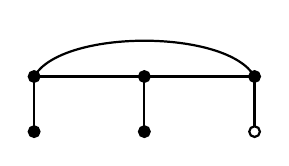
\begin{tikzpicture}[scale=.7,style=thick,x=1cm,y=1cm]
\def\vr{2.75pt}
\path (0,0) coordinate (v2);
\path (0,1) coordinate (v3);
%  edges
\draw (v2) -- (v3);
%%%%%%%%%%%%%%
\path (2,0) coordinate (u2);
\path (2,1) coordinate (u3);
%  edges
\draw (u2) -- (u3);
%%%%%%%%%%%%%%
%%%%%%%%%%%%%%
\path (4,0) coordinate (w2);
\path (4,1) coordinate (w3);
%  edges
\draw (w2) -- (w3);
%%%%%%%%%%%%%%
%%%%%%%%%%%%%%
\draw (v3) -- (u3);
\draw (u3) -- (w3);
%
\draw (v2) [fill=black] circle (\vr);
\draw (v3) [fill=black] circle (\vr);
%
\draw (u2) [fill=black] circle (\vr);
\draw (u3) [fill=black] circle (\vr);
%
%
\draw (w2) [fill=white] circle (\vr);
\draw (w3) [fill=black] circle (\vr);
%
\draw (v3) to[out=60,in=120, distance=1cm ] (w3);
%%%%%%%%%%%%%%
\end{tikzpicture}

\end{document}